\section[TV Cell Model]{Tuberculoventral Cell Model: Fitting Tone and Noise Rate Level Curves}

\subsection{Background}

TV cells are characterized as having a non-monotonic response to tones with increasing sound level and respond poorly to broadband noise \citep{SpirouDavisEtAl:1999,NelkenYoung:1997,ReissYoung:2005}, as shown in Fig.~\ref{fig:SpirouFig8}.

% \begin{figure}[htb]
% \centering
% % \resizebox{5in}{!}{\includegraphics[angle=-90]{NoFigure}}
% 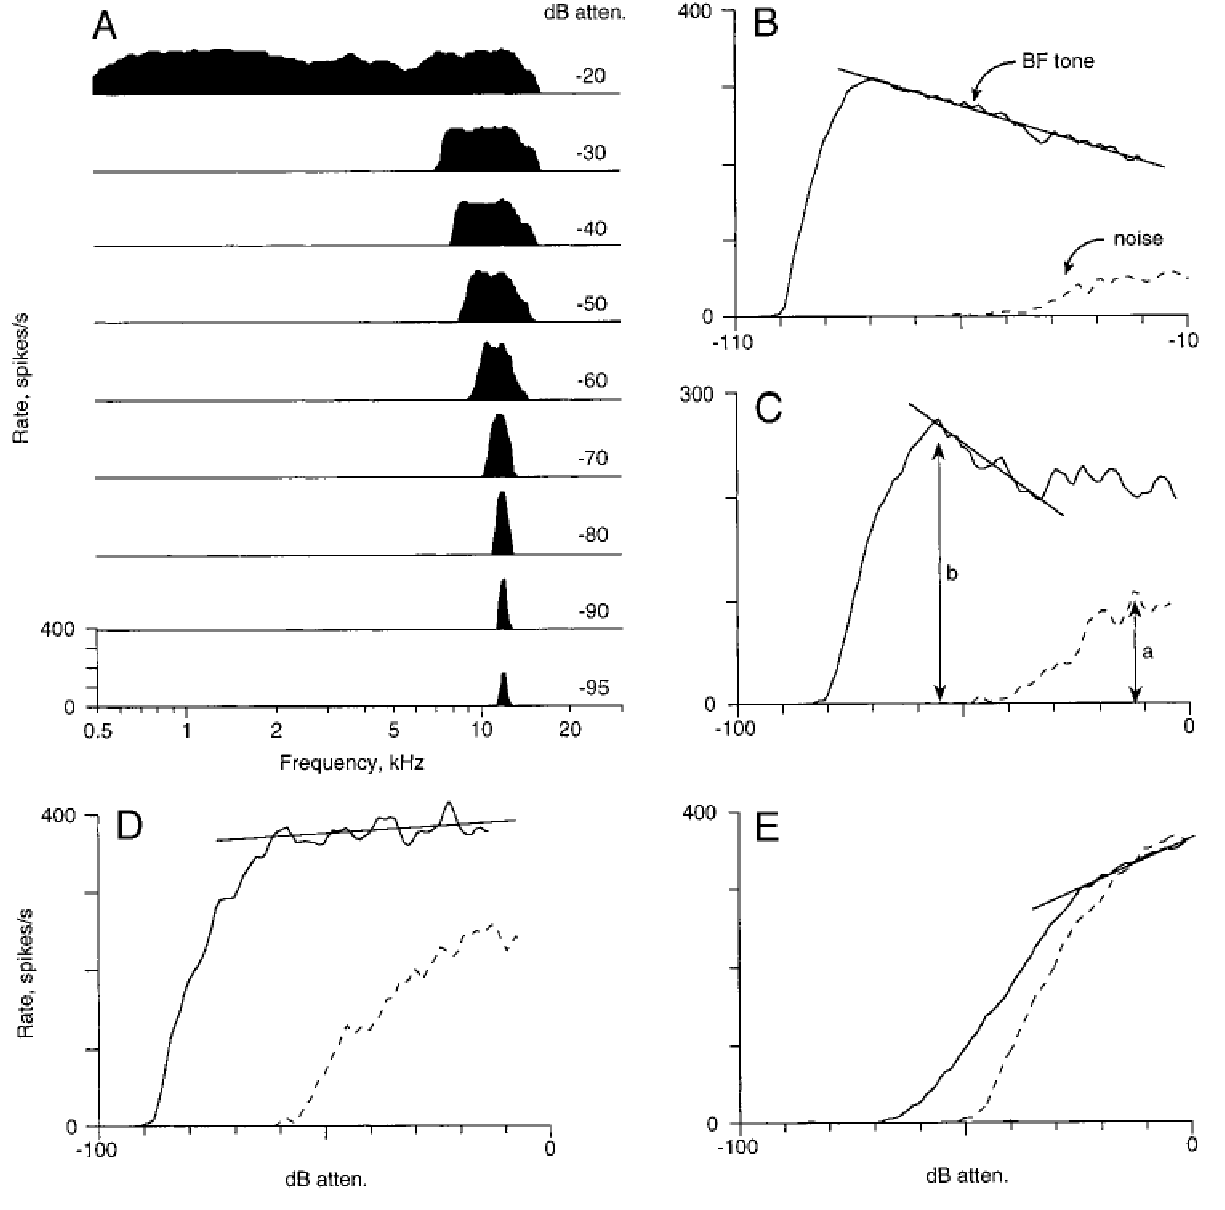
\includegraphics[keepaspectratio,width=0.8\textwidth]{Spirou-Fig1-type2}
% \caption[Experimental data of a single Type-II~DCN~unit]{Experimental data of a single Type-II~DCN~unit \citep[Fig.~1]{SpirouDavisEtAl:1999}.
% \yellownote{Figure~\ref{fig:SpirouFig1} needs permission}}
% \label{fig:SpirouFig1}
% \end{figure}


\TV~or vertical cells are glycinergic, inhibitory cells found in the deep layers of the \DCN~that send axon collaterals to the \VCN\@.
They are characterized as having a non-monotonic response to tones with increasing sound level and respond poorly to broadband noise \citep{SpirouDavisEtAl:1999,NelkenYoung:1997,ReissYoung:2005}, as shown in Fig.~\ref{fig:SpirouFig1}.
Anterograde labeling in the \DCN~suggests \TV~cells project tonotopically to the \VCN~not just on-CF, but also to the low and high frequency side bands \citep{MunirathinamOstapoffEtAl:2004,OstapoffMorestEtAl:1999}.
With retrograde labelling in the \DCN~three types of ventro-tubercular units in rats were identified \citet{FriedlandPongstapornEtAl:2003}, as apposed to only two types in cats \citep{SmithRhode:1989,OertelWuEtAl:1990}.
These units are identified as \TS~and \DS~cells, with the third in rats identified as small adendritic neurons.


Ultra-structural labeling of synapses in the rat \DCN~suggest \TV~cells are inhibited by glycinergic \DS~cells and from sources in the \DCN~but excitatory inputs were not found from \TS~cells in the rat \citep{Rubio:2005}.
Evidence in the mouse suggests otherwise since intracellular responses from labeled \TV~cells in the mouse show clear excitatory input from \TS~cells and diffuse inhibitory input from \DS~cells \citep{ZhangOertel:1993b,WickesbergOertel:1993}.

%\smallskip{}


%\TV cells receive mono-synaptic excitatory input from auditory nerve fibres \citep{OertelWu:1989,ZhangOertel:1993b}.
Taken together, these results suggest that auditory nerve fibres (predominantly \LSR fibres) form the major excitatory input to type~II DCN units along with other excitation from TS cells.
If true, this hypothesis could also explain the finding that type~II DCN units have consistently higher thresholds than \DCN~principal cells \citep{YoungBrownell:1976} because \LSR~auditory nerve fibres also have elevated thresholds relative to the lowest threshold auditory nerve fibres \citep{Liberman:1978}.
However, patterns of auditory nerve innervation of the \DCN~are most consistent with \HSR~fibre innervation of \TV~cell somata and \LSR~fibre innervation of dendrites \citep{Liberman:1993}.
In that case, the low spontaneous rates and high sound thresholds of type II DCN units might be caused by a high intrinsic electrical threshold \citep{HancockDavisEtAl:1997}; this is consistent with the responses of vertical cells to intracellular current injection \citep{DingVoigt:1997,ZhangOertel:1993b}.

%\smallskip{}

Type~II units also supply an inhibitory input to the \VCN~\citep{WickesbergOertel:1990}, but the role of type~II terminals in the \VCN~is less clear.
Three different hypotheses have been raised.
The first is that this projection modulates the response thresholds of \VCN~neurons \citep{PaoliniClark:1998}.
The role of type~II units in spectral processing is that of a narrowband inhibitor. Responses of \DCN~principal cells are strongly inhibited by this narrowband source.
As a result, \DCN~principal cells are inhibited by sharp spectral peaks close to their \BF~\citep{SpirouDavisEtAl:1999}.

%\smallskip{}



\subsubsection{Modeling of Tuberculoventral cells}

\yellownote{Expand previous studies  of the DCN incl. TV cells}
\citet{ArleKim:1991a} were the first to show type~II \EIRA  with simple McCullock-Pitts point neuron models.
\textit{(From Hancock Davis Voigt 97) Blum et al. (1995) used a wideband inhibitory   mechanism to create type II unit responses in a model of the DCN. In that   model, each cell population was described by a mathematical formula for its   steady-state rate-level function. This level of abstraction was used to focus   specifically on the role of network connectivity in determining the   steady-state behavior of DCN units. The level of abstraction employed in our   model allows for examination of temporal response properties including PST   histograms and cross-correlation analysis.}
\citep{DunnVetterEtAl:1996} performed some modelling.


Modeling of Type~II units in the \DCN~has been thoroughly categorised by Davis and colleagues \citep{YoungDavis:2002,HancockDavisEtAl:2001,DavisYoung:2000,SpirouDavisEtAl:1999,HancockDavisEtAl:1997,DavisVoigt:1996,DavisVoigt:1994,DavisVoigt:1991}.
Low spontaneous rate is created in a neural model by either increasing the intrinsic spiking threshold or lowering the synaptic strength of the inputs.
Intracellular observations in decerebrate gerbils show higher thresholds in type~II units \citep{DingVoigt:1997}; and observations of hyperpolarisation responses to off \gls{BF}~tones in intracellularly recorded type II units.

Another case for type II behaviour of no spontaneous activity, is a preference of \LSR, high threshold \AN~fibres over \HSR~fibres to synapse with \TV~cells.
Whether \LSR~fibres preference the deep layers of the \CN~are yet to be confirmed \citep{Ryugo:2008,MeltzerRyugo:2006,RyugoParks:2003,BabalianJacommeEtAl:2002}.

%\smallskip{}

%\citep{Rhode:1999} Vertical cells in gerbils (mainly type III)

%\smallskip{}

The intrinsic mechanism is more favourable in Type II units, provided there is sufficient inhibition and excitation \citep{HancockDavisEtAl:1997}.
Lateral inhibition was disregarded in favour of wide-band inhibition \citep{HancockDavisEtAl:1997} and is favoured in this model.
Work by Reed and Blum \citep{ReedBlum:1995,BlumReedEtAl:1995,ReedBlum:1997,BlumReed:1998} on the circuitry of the \DCN~showed that wide-band inhibition was necessary for the principal cells of the \DCN~including type II units.
 %\smallskip{}


%\yellownote{The above paragraphs need to be cleaned up and worked into the idea of generating BNN models using a simple approach}
%\smallskip{}

% \subsubsection{Key design factors}


% \textbf{Morphological}
% \begin{itemize}
% \item vertical/multipolar cell in deep layer of \DCN~\citep{Rhode:1999}
% \item receive small number of \ANF~syn to dend
% \item receive large number of Gly and \GABA~syn to soma and dendrite
% \end{itemize}





% \begin{itemize}
% \item Rat model (no \TS-TV) but has been shown in other mammals
% \item Unable to include other \DCN~inputs
% \item Model must show \DSTV~inhibition and offset of distribution

% \item Notch noise stimulus $\rightarrow$ need more \TV~cells across frequency
% \item Input \SPL~and weight of excitation affect spiking output
% \item Larger network $\rightarrow$ increased computational load
% \item Solution: Parallelism model
% \end{itemize}



\subsection{Implementation}


\begin{figure}[htb]
\centering
% \resizebox{5in}{!}{\includegraphics[angle=-90]{NoFigure}}
\resizebox{0.6\textwidth}{!}{\includegraphics{TV_RateLevel_Fig8.eps}}\\
\caption[Experimental data of a single Type-II~DCN~unit]{Experimental tone and BBN rate-level data of a single Type-II~DCN~unit \citep[Fig.~8]{SpirouDavisEtAl:1999}.}\label{fig:SpirouFig8}
\end{figure}



%%% Local Variables:
%%% mode: latex
%%% mode: tex-fold
%%% mode: visual-line
%%% TeX-master: "SimpleResponses"
%%% TeX-PDF-mode: nil
%%% End:
